\chapter{Methodology}
\label{chap:methodology}



In this chapter, we explain the general approach to carry out the attack. First, we give an overview of the attack's procedure. Then, we explain each step separately in the remaining sections. 
\\
\\

Regardless of the smartwatch, we can break down the attack into 5 stages: 

\begin{enumerate}
    
    \item \textbf{Application Selection}. In the first stage, the attacker selects which applications he wants to target according to his objectives.
    
    \item \textbf{Data Generation} The Data Generation consists of repeatedly triggering actions related to an application on a smartwatch and recording all the traffic traces generated by these actions.
    
    \item \textbf{Feature Extraction} This stage consists of extracting statistical features from the traffic trace that best characterize the traffic and would enable fingerprinting.
    
    \item \textbf{Model Selection}. In this phase, we select the model that best fits the data. 
    
    \item \textbf{Evaluation}. The Evaluation is the final stage and reflects how well the model performs.
    
\end{enumerate}

Fig. \ref{fig:attack_p1} shows graphically all the stages of the attack

\begin{figure}[H]
 \centering
 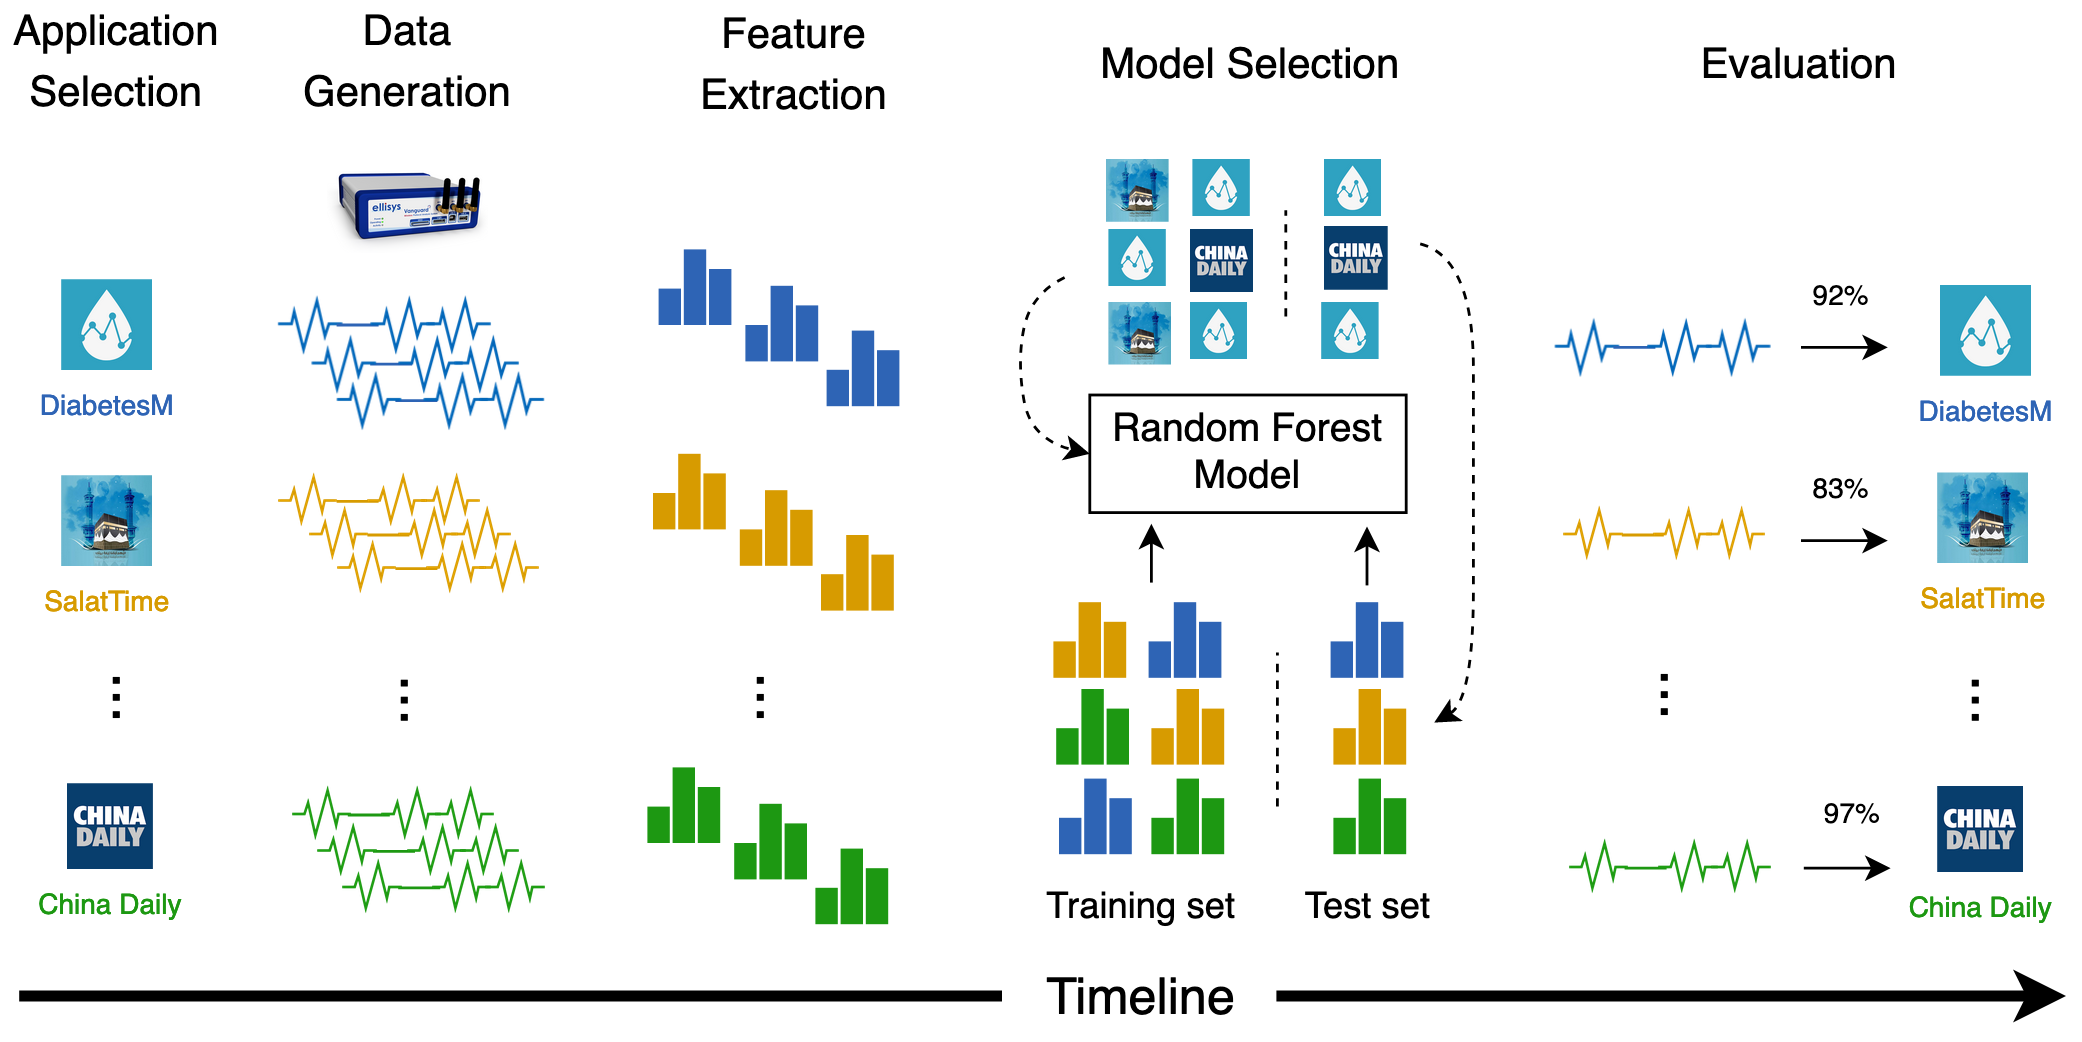
\includegraphics[width=0.98\textwidth]{figures/methodology.png}
 \caption{Attack broke down into 5 stages}
 \label{fig:attack_p1}
\end{figure}


 In the remaining sections, we describe each stage based on one particular smartwatch-phone pair: \textbf{Huawei-Pixel} from which specifications can be found in Tab.~\ref{tab:main_watch_spec}. Nevertheless the general approach applies for other smartwatch-phone pairs. 



\section{Application and Action Selection}
\label{sec:application_and_action_selection}
Applications are chosen based on three criteria:

\begin{itemize}
  \item \textit{Confidentiality}: Applications bearing specially sensitive information. Such as Health or Religious related applications, but also application that could show political interests or information about ethnicity.
  \item \textit{Popularity}: Popular applications based on the number of downloads and reviews, but also apps listed on famous websites that rank best smartwatches applications \cite{bestWearOSApp, bestWearOSApp2}.
  \item \textit{Nativity}: Applications installed by default on the smartwatch.
  \end{itemize}
  
Popularity and nativity ensure that the selected applications are representative of which application is more likely to be triggered, while confidentiality shows that the attack also works for specific sensitive targeted applications. Tab.~\ref{tab:app_examples} shows examples of selected applications, installed on the Huawei smartwatch, along with a short description and the selection criteria.
\\


\begin{table}[h]
\centering
 \begin{tabular}{@{}llll@{}} 
 \toprule
 Application & Description & Criteria  & Type\\ [0.5ex] 
 \midrule
 DiabetesM & Diabete Manager & Confidentiality & Health \\ 

 Maps & Google GPS navigation system & Popularity & Map \\

 Weather & Weather forecast  & Nativity & Other \\

 Spotify & Music Streaming & Popularity  & Other \\

 SalatTime & Islamic Prayer Manager & Confidentiality & Religious \\ 
 \bottomrule

\end{tabular}
\caption{Sample of selected applications installed on Huawei smartwatch with a short description, the criteria of selection and the application's type}
    \label{tab:app_examples}
\end{table}


We selected a total of 55 applications for our main stream experiment on the Huawei smartwatch. The complete list of these applications is given in the Appendix Tab.~\ref{tab:initial_Apps}. Fig.~\ref{fig:app proportio} shows the proportion of applications selected wrt. their criteria and types. We see that the most represented types of applications are Fitness apps and Health related apps, which is typically the kind of applications one would find on her smartwatch.

\begin{figure}[h]
\centering
\begin{subfigure}{.5\textwidth}
 \centering
  \includegraphics[width=0.65\linewidth]{figures/plots/Apps criteria repartition.png}
  \label{fig:sub1}
\end{subfigure}%
\begin{subfigure}{.5\textwidth}
  \centering
  \includegraphics[width=0.95\linewidth]{figures/plots/Apps typle repartition unfiltered.png}
  \label{fig:sub2}
\end{subfigure}
\caption{\textbf{Left:} Proportion of applications by criteria. \textbf{Right:} Proportion of applications by types}
\label{fig:app proportio}
\end{figure}


While the action of opening the application for the 55 initially installed application comes for free, we selected 17 extra actions on specific applications; we call them \textbf{in-app} actions. A complete list of these actions is given in the Appendix (see Tab. \ref{tab:selected_actions}).





\section{Data Generation}
\label{sec:data_generation}

We designed and implemented a system that allows an attacker to automatically generate a dataset from the applications selected in the previous stage. This automation system uses 5 devices:

\begin{itemize}
  \item \textit{Bluetooth Recorder}: Records Encrypted Bluetooth traces.
  \item \textit{Central Controller}: Orchestrates the simulation by synchronizing and controlling captures of Bluetooth traces and actions performed on the smartwatch.
  \item \textit{Bluetooth Recorder Controller (BR Controller)}: Controls the Bluetooth Recorder via a software.
  \item \textit{Smartwatch}: Performs application's action.
  \item \textit{Smartphone}: The Smartwatch's paired phone. 
\end{itemize}


\subsection{Automation Setup} We created a WLAN with no internet connection over Wi-Fi that connects the Central Controller to the smartwatch and the BR Controller. The BR Controller is connected via USB cable to the Bluetooth Recorder. The smartwatch is also connected to a smartphone via Bluetooth. Finally, we connect the smartphone to another WLAN via Wi-Fi with internet connectivity. This setup forces the smartwatch to use the phone as a default gateway over Bluetooth to access the internet while still being able to receive commands from the Central Controller via Wi-Fi. The setup is depicted in Fig. \ref{fig:automation_testbed}. 


\begin{figure}[H]
 \centering
 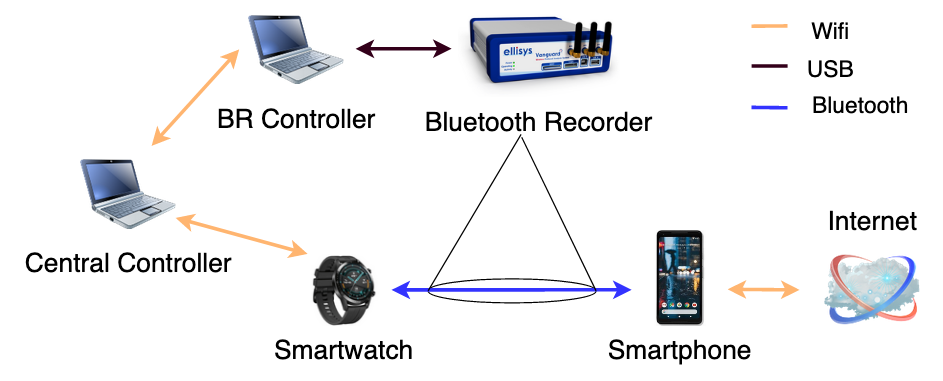
\includegraphics[width=0.7\textwidth]{figures/automation_testbed.png}
 \caption{Automation architecture.}
 \label{fig:automation_testbed}
\end{figure}

\\
\\

We specify that the smartwatch is charging at all time during data generation to ensure that it does not run out of battery, but also to allow persistent Wi-Fi connectivity, as we discussed in Sec.~\ref{sec:smartwatches}.
\\

While we change the smartwatch and smartphone for different experiments, we keep the same Bluetooth Recorder, BR Controller and Central Controller across experiments. We use Ellisys Vanguard BV1 for the Bluetooth Recorder, a Dell running Window 10 for the BR Controller having Ellisys Bluetooth Analyzer software installed and a ThinkPad running Ubuntu Bionic for the Central Controller.



\subsection{Automation Flow} For each action that is targeted by the attacker, the automation goes as follows. First, the Central Controller sends to the BR Controller the command to start recording the Bluetooth traffic of the targeted smartwatch-phone pair. Upon receiving the confirmation that the capture started by the BR Controller, the Central controller starts executing the action on the smartwatch. Once the action is done, the Central controller waits for a few seconds to ensure that the Bluetooth communication is finished. Then, the Central Controller sends a command to the BR Controller to stop and save the capture with the name of the application and the action which becomes the label of the capture. After having received the confirmation that the capture is saved, the Central controller sends a force-stop\footnote{\textbf{\textsc{force-stop}} ensures that the application is fully stopped and is ready for a fresh restart. We are convinced that this does not influence the real behavior of application loading since we can safely assume a garbage collector inside the smartwatch responsible of stopping left over processes after some period of time.} command such that the application is stopped and then waits a few seconds to ensure that the traffic reach a steady state. This procedure is repeated as many times as the attacker wants samples per action before switching to another action.


\subsection{Implementation}
On one side, we used \texttt{adb}\footnote{\textbf{\texttt{android debug bridge (adb)}} is a CLI tool that let a remote machine access an android device.} and \texttt{monkeyrunner}\footnote{\textbf{\texttt{monkeyrunner}} is a python API running on \texttt{Jython}. It provides simplified command to execute commands on an Android device.} on the Central Computer to control the smartwatch remotely. And on the other side, we used the python library \texttt{socket} to implement a server on the BR Controller which waits for commands sent by the Central Computer. The BR Controller uses \texttt{autoIt3}\footnote{\textbf{AutoIt Scripting Language} is a scripting language used to automate the interaction with the Windows GUI.} to execute the command on the Bluetooth Recorder software. The automation system runs checks (e.g. Bluetooth connection is up) to record any failure that might occur during the automation and keeps a log record.
\\

The whole system is composed of 1,350 Line of Code (LoC). 1,070 LoC run on the Central Controller: 620 python LoC and 550 yaml encoded commands to perform action on the smartwatch. On the other end, 280 LoC run on the BR Controller: 180 python LoC for the server and 100 AutoIt3 to automate commands on the software controlling the Bluetooth Recorder.

\subsection{Benefits}
The most important benefit from the automation system is the time consumption. We measured that to perform one capture, our automation system takes approximately one minute. If we assume an adversary that can generate capture as fast as the automation system, and has selected 24 actions with 25 samples per action, it would take him 10 hours in the data collection process. The time saving results in an easier dataset scalability and maintainability for an attacker. Moreover, the system is not prone to inattention error that human can have and thus might lead to a cleaner dataset. 
\\

We highlight that the system we designed is not only bounded to capture traffic between smartwatches and mobile phone. It can also be used to capture various kind of traffic. For instance, the system could be applied to audio fingerprinting, where the smartwatch would be replaced by the smartphone and the smartphone by earphones in Fig.~\ref{fig:automation_testbed}.

\subsection{Limitations and Alternatives}
The automation system only works on Android and WearOS. Unfortunately, \texttt{adb} and \texttt{monkeyrunner} are not available for other Operating Systems. Still, other alternatives exist. Tizen, running on Samsung devices, allows a remote connection with \texttt{sdb} (Smart Debug Bridge). However, the interaction with the smartwatch is much more constrained and allows only the command to open applications. 
\\


There are actions that the automation system is unable to control. For instance, if a push notification arises on the watch generating extra traffic, the system won't be able to detect it. The same goes for background updates. This results in noisier captures. There is still an option to filter out this extra noise by fetching the \texttt{btsnoop} log file on the smartwatch. However, we decided to not use this method as it might have significant discrepancies with the actual traffic sent, and also because not all smartwatches support \texttt{btsnoop}. We also note that keeping this background noise is a more realistic scenario of what we would find in the wild.
\\


Finally, automated actions might fail to capture real user pattern actions. However, this would also be true if a single user performs actions: the traces might be too specific to that user. 




\section{Feature Extraction}
\label{sec:Feature extraction}
In this section, we explain the third stage of the attack

\subsection{Basic Features Extraction} From our threat model, the attacker cannot see the payload's content of the traffic. However, nothing prevents him from passively recording, for each packet, the following characteristics: 
\begin{itemize}
    \item \textit{Direction}: The packet's direction. Either incoming (from phone to smartwatch) or outgoing (from smartwatch to phone).
    \item \textit{Length}: The packet length.
    \item \textit{Timing}: The time at which the packet is sensed by the attacker.
\end{itemize}{}


While the attacker can also see the Bluetooth packet type, we decided to not use this information because the Bluetooth protocol stack on smartwatches is in principle implemented on the Bluetooth chip and on the device's OS and thus is independent of applications.


\subsection{Statistical Features Extraction} 
From packets described by the tuple (\textit{Direction}, \textit{Length}, \textit{Timing}), we extracted statistics based on packet length and packet arrival time for each capture traces.
\\
 
 For packet length, we formed three groups: incoming packets only, outgoing packets only and non-null packets. On each group of packets, we computed the following six statistical quantities: The minimum, maximum, mean, standard deviation, number of packets in the group and the kurtosis\footnote{The kurtosis measures how heavily tailed is a distribution.}. In addition, we created features for each unique packet length, and by grouping the count of these unique packet length, we also computed the 6 statistical values above.
 \\
 
 For packets arrival time, we extracted the inter-arrival-time (IAT) between each packet having size more than 0, 46 and 1,005 length (see Sec.\ref{sec:model selection}). From these extracted IAT values, we also computed the same six statistical values.
 \\
 
 At this point, we are left with $6*3 + 1,005 + 6 = 1,029$ features on packet length and $3*6=18$ features on timing, thus a total of 1,047 features.
 \newpage



\section{Model Selection}
\label{sec:model selection}
In this section, we present the characteristics of the model.

\paragraph{Classifier.}
We use the \texttt{RandomForestClassifier} from the python library \texttt{sklearn}. Choosing Random Forest was motivated by the fact that this model is well known in traffic-fingerprinting to provide good performance~\cite{10.1145/3274694.3274697, k-fingerprinting, taylor2016appscanner}, but also, because it can deal well with high-dimensional data with sparse features and it gives an easy way to understand the importance of features. We set no restriction on the maximum depth of trees, Gini impurity for the splitting criteria, and the number of features to be considered in a split to the square root of the maximum number of features. We tuned these parameters by running a grid search algorithm and a cross-validation score. We also set the number of trees in the forest to 200.

\paragraph{Feature Filtering.} We setup the range of the unique packet length from 46 to 1,005. 1,005 is the maximum packet length in bytes that a Bluetooth packet can have. 46 was found by performing a grid search where we withdrawn each unique packet length feature from 1 to i until until i = 110. Since we got a stable accuracy until i=46 before dropping significantly, we expect that packets having length less than 46 are mostly controlled packets not related to applications. To further filter features, we leverage the RF architecture to extract the feature importance and filtered out all features with null importance. Consequently, we reduced the initial 1,047 features to less than a half. This allowed us to have a better insight of the features and speed up training and predictions from around 10\% to 40\%. 








\section{Evaluation}
\label{evaluation}

For each experiment, we follow the same guideline to evaluate the model: We first perform equalization across classes to ensure that all classes are perfectly balanced. We then performed 50 random split cross-validation with 75\% train and 25\% test to compute the accuracy and the 95\% confidence interval\footnote{computed as two times the standard deviation.} averaged over all predictions. Finally, we plot a confusion matrix of one realisation to gain more insight about the classifier.
